\section{Anticipating and executing financial dependencies}
\label{sec:execution}

\subsection{A complete account of encountered debts}
Of 188 episodes requiring explicit financing, 128 end in payment and sixty in elimination. Payment entails 180 mortgages and 89 building-sale actions to meet \$51,997 in obligations. Sixty-seven payments require one action and sixty-one require two to ten. No successful payment uses an engine fallback. All four configurations complete multi-action sequences, although their encountered obligations differ.

Historical feasibility checks identify three further payable debts that end in declaration. Thus 128 of 131 demonstrated-payable debts are paid. Fifty-six other eliminations exceed the generous own-asset bound. The remaining case, G7 Opus, has \$1,310 in nominal finance against a \$750 debt but only \$440 reachable under the supplied menu. The empty bank house stock leaves no offered hotel sale. This distinguishes asset accounting from the available sequence, rather than asserting impossibility under every Monopoly implementation.

The payment fraction provides the population context. Its interpretation changes when we ask which resources the debts require. Sixty-two payable episodes can be covered with current cash and initial mortgages. Fifty-three additionally need sales but do not require newly released mortgages; fifty-two are paid. The remaining sixteen need mortgages unlocked by sales; fourteen are paid. Figure~\ref{fig:finance} displays this partition. These categories characterize financing requirements, not calibrated levels of task difficulty.

\begin{figure*}[t]\centering
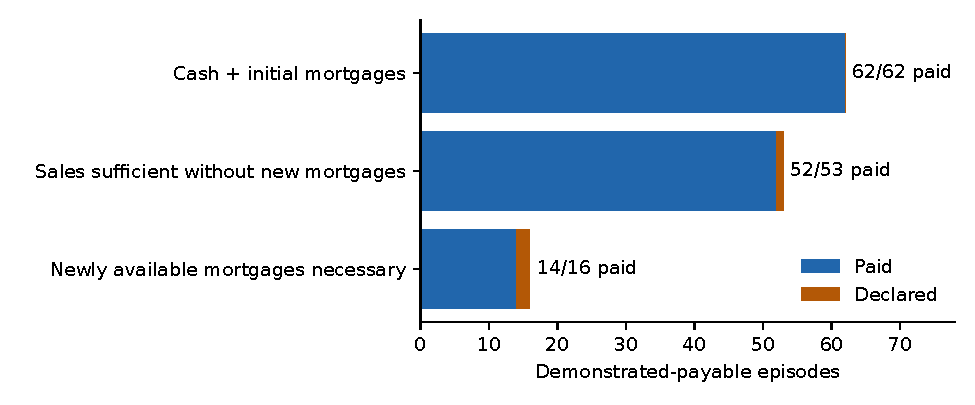
\includegraphics[width=.88\textwidth]{debt_requirements.pdf}
\caption{The 131 demonstrated-payable episodes by required resource class. Actual payment establishes 128 routes; historical legal sequences establish the other three. Newly released mortgages are necessary when even cash, all salvage and initial mortgages fall short. The other 57 eliminations are outside this figure.}\label{fig:finance}
\end{figure*}

\subsection{Prospective assessment when initial options are insufficient}
In nineteen successful payments, agents sell buildings and then use one or more of 33 mortgages absent from the first menu. Fourteen of these payments meet the necessity condition $U_0<D\leq U_*$. Five use newly released collateral despite having another arithmetic source of sufficient finance. Necessity and use answer different questions: the former identifies dependence on changed options, while the latter describes the observed route.

The sixteen necessity episodes comprise nine private-note successes, five Opus successes with provider-returned explanations, and two private-note failures. Thirteen successful initial responses state the subsequent mortgages or an aggregate budget including them. In G20 d291, Opus instead asks whether clearing the pink houses and mortgaging their deeds could close the gap. It then carries out payment. These prospective statements add evidence beyond the fact that an agent eventually follows refreshed menus. They remain recorded statements, not a measurement of the computation producing the action.

Both failures declare at the first menu. In G12 d190, Sol totals \$53 cash, \$225 salvage and \$130 in listed mortgages, obtaining \$408 against \$500 owed. Selling the red buildings also releases \$340 in mortgages, which the sum omits. In G17 d234, Gemini totals \$500 salvage and a \$30 Baltic mortgage against \$550 owed, omitting \$375 in released dark-blue collateral. The same systems succeed in other necessity episodes: Sol pays two of three and Gemini five of six; Opus pays five of five and Grok two of two. These are two omissions within a population containing successful dependency assessment, not a universal boundary of either model.

\TranscriptTitle{g20-payment}{An announced budget survives ten actions}
Only Sol and Gemini remain in G20. Gemini raises Pennsylvania's rent to \$1,400 after estimating Sol's total liquidation resources at \$1,414. Sol lands there with \$49, nine orange houses and two brown hotels:
\TranscriptQuote{g20-d327-plan}
Sol sells its development in two actions and mortgages eight deeds. At the last mortgage:
\TranscriptQuote{g20-d336-last}
The events record \$700 from sales and \$665 from mortgages, giving $49+700+665-1,400=14$. Gemini's aggregate estimate was also correct, although its salvage and mortgage components offset by \$25. The episode establishes a stated financing target followed by the corresponding payment and remainder. Updated menus remain available throughout; ten executed actions are not ten demonstrated levels of lookahead.
\TranscriptSource{G20 d325, d327--336, standard responses. Quoted fields are Sol's private notes. They are not messages exchanged with Gemini. Payment and final cash are checked against events and the next prompt.}

The third payable declaration has different evidence. In G12 d249, Grok owes \$250 with \$43 and seven pink houses. Its private note recognizes a sale-based payment route, assistant content names a sale, but the received call declares bankruptcy. That action ends play before any sale. The distinction matters: the two necessity failures omit a financing resource in their stated sums, whereas this record contains a payment assessment that conflicts with the applied action.

\subsection{Investment and subsequent ownership}
Finance also determines what an agreement becomes. Sol and Gemini build in the first management turn after trade completion on 16/17 and 17/18 groups; Opus and Grok do so on 7/15 and 3/13. The twenty other windows include nine groups with no build option for that group, four engine defaults, four calls conflicting with content and three other valid ends. A missing current build option can coexist with a possible redemption-and-build sequence. The categories therefore distinguish offered actions, stated financing choices and execution rather than labeling every non-build a preference to wait.

These ownership histories provide the stakes of bargaining. Trade-completed groups collect \$57,378 before loss or game end, with \$53,810 collected by groups built in the first window. Receipts reflect development, subsequent landings, holding time and selection; they are not incremental investment returns. Thirty-eight of forty nonterminal eliminations follow rent on the creditor's developed color property. Estates then move 227 deeds and complete 52 groups during play. A further 69 completions occur only at final elimination. The later incidents use these pathways to explain what participants describe as worth financing or preventing.
